\documentclass[arhiv]{../izpit}
\usepackage{fouriernc}
\usepackage{xcolor}
\usepackage{tikz}

\begin{document}

\izpit{Programiranje I: 3.\ izpit}{5.\ september 2016}{
  Čas reševanja je 150 minut.
  \textbf{Funkcij v Haskellu ne pozabite opremiti z ustrezno signaturo.}
  Veliko uspeha!
}

%%%%%%%%%%%%%%%%%%%%%%%%%%%%%%%%%%%%%%%%%%%%%%%%%%%%%%%%%%%%%%%%%%%%%%

\naloga[Ljudožerci in padalci, 20 točk]

Nalogo lahko rešujete v Haskellu ali v Pythonu.

\vspace{0.5\baselineskip}\noindent
Na neki dolgi cesti stoji $n$ ljudožercev, pri čemer $i$-ti ljudožerec stoji na koordinati $x_i$. Začetne koordinate
ljudožercev lahko predstavimo s seznamom $[x_1, x_2, \ldots, x_n]$, pri čemer velja $x_i \leq x_{i+ 1}$ za $i = 1, \ldots, n - 1$.
Na to cesto se bo, eden za drugim, spustilo $m$ padalcev, pri čemer bo $j$-ti padalec pristal na koordinati $a_j$. Po pristanku padalec
pomaha najbližjemu ljudožercu. Če je takšnih več, izbere tistega z manjšo koordinato. Če je tudi takšnih več, je vseeno,
katerega izbere. Ljudežerec se bo sprehodil do padalca, ga požrl in ostal na koordinati $a_j$. Napišite funkcijo, ki kot argumenta
dobi urejen seznam števil $[x_1, x_2, \ldots, x_n]$ ter seznam (ne nujno urejen) števil $[a_1, a_2, \ldots, a_m]$.
Funkcija naj vrne urejen seznam, ki vsebuje končne koordinate ljudožercev (stanje po tem, ko bodo pristali vsi padalci). Primer:

\begin{verbatim}>>> ljudozerci([1, 4, 4, 6, 10, 11, 15], [3, 5, 4, 8, 4, 14])
[1, 4, 5, 8, 10, 11, 14]
\end{verbatim}

\noindent
Funkcija naj ima časovno zahtevnost $O(m \log n)$. 


%%%%%%%%%%%%%%%%%%%%%%%%%%%%%%%%%%%%%%%%%%%%%%%%%%%%%%%%%%%%%%%%%%%%%%
\naloga[Koruza, 20 točk]

Nalogo lahko rešujete v Haskellu ali v Pythonu.

\vspace{0.5\baselineskip}\noindent
V neki deželi imajo koruzo, katere stebla zrastejo visoko v nebo (tudi po več kilometrov). Na tej rastlini zraste mnogo
koruznih storžev na različnih višinah. Hobit, ki rabuta koruzne storže, bi si jih rad nabral kar največ. Ker se hobit pri plezanju
utrudi, ne bo nujno uspel pokrasti vseh. Za vsak preplezani meter navzgor porabi eno enoto energije. Pri plezanju navzdol
potroši zanemarljivo malo energije. Pred začetkom podviga ima Hobit $h$ enot energije. Napišite funkcijo, ki izračuna
največjo število storžev, ki jih lahko Hobit nabere. Vsaka rastlina je podana s seznamom števil oblike
$[x_{i,1}, x_{i,2}, \ldots, x_{i, a_i}]$, kjer je $a_i$ skupno število strožev na $i$-ti rastlini, cela števila $x_{i,1}, \ldots, x_{i,a_i}$
pa so višine (v metrih) posameznih storžev. Veljalo bo $x_{i,1} \leq x_{i,2} \leq \cdots \leq x_{i,a_i}$. Funkcija kot argumenta
dobi število $h$ in seznam seznamov $[[x_{1,1}, x_{1,2}, \ldots, x_{1, a_1}], \ldots, [x_{n,1}, x_{n,2}, \ldots, x_{n, a_n}]]$, kjer
je $n$ število rastlin. Primer:

\begin{verbatim}>>> rabutanje(10, [[2, 5, 9], [5, 6, 7, 8], [1, 3, 6]])
5
\end{verbatim}
%
Hobit lahko nabere najnižji storž s prve rastline in vse storže z druge rastline, torej skupno 5 storžev. Pri plezanj bo porabil
vso razpoložljivo energijo.

\vspace{0.5\baselineskip}\noindent
\textit{Namig (1.\ način):} Naj bo $f(i, j)$ največje število storžev, ki jih lahko nabere, če pri plezanju po rastlinah $1, 2, \ldots, i$ porabi $j$
enot energije. Ali znate učinkovito izračunati $f(n, h)$? 

\vspace{0.5\baselineskip}\noindent
\textit{Namig (2.\ način):} Naj bo $g(i, j)$ najmanjša količina energije, ki jo potrebujemo, če pri plezanju po rastlinah $1, 2, \ldots, i$ naberem
skupno $j$ storžev. Ali znate učinkovito izračunati največji $s$, za katerega velja $g(n, s) \leq h$? 


%%%%%%%%%%%%%%%%%%%%%%%%%%%%%%%%%%%%%%%%%%%%%%%%%%%%%%%%%%%%%%%%%%%%%%
\naloga[Podjetje, 40 točk]

V nekem podjetju so uslužbenci urejeni hierarhično, tj.\ strukturo zaposlenih lahko predstavimo z drevesom. Vsak zaposleni (razen
direktorja) ima natanko enega neposrednega šefa. Uslužbenci imajo pod seboj lahko več neposredno podrejenih. V Haskellu to
predstavimo s podatkovnim tipom:
\begin{verbatim}
data Drevo = Drevo String [Drevo]
\end{verbatim}
Na primer, drevo
\[
  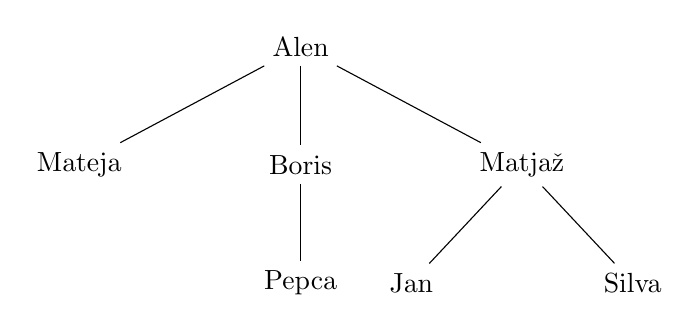
\begin{tikzpicture}[sibling distance=8em]
    \node (d) {Alen}
      child {node {Mateja}}
      child {node {Boris}
        child {node {Pepca}}
      }
      child {node {Matjaž}
        child {node {Jan}}
        child {node {Silva}}
      }
    ;
  \end{tikzpicture}
\]
bi predstavili kot
\begin{verbatim}
let d = Drevo "Alen" [
  Drevo "Mateja" [],
  Drevo "Boris" [Drevo "Pepca" []],
  Drevo "Matjaž" [Drevo "Jan" [], Drevo "Silva" []]
]
\end{verbatim}

\podnaloga[10 točk]
Nekemu uslužbencu $x$, njegovemu šefu, šefu šefa itd. pravimo \emph{veriga} uslužbenca $x$.
Sestavite funkcijo % \begin{verbatim}veriga :: a -> Drevo a -> [a]
% \end{verbatim}
\verb|veriga|, ki prejme ime zaposlenega in drevo ter vrne seznam z imeni vseh v njegovi verigi. Zgled:
\begin{verbatim}Prelude> veriga "Pepca" d
["Pepca","Boris","Alen"]
\end{verbatim}


\podnaloga[10 točk]
Nekemu uslužbencu $x$ in vsem njegovim (posredno ali neposredno) podrejenim pravimo \emph{ekipa} uslužbenca $x$.
Sestavite funkcijo
% \begin{verbatim}ekipa :: Ord a => a -> Drevo a -> [a]
% \end{verbatim}
\verb+ekipa+, ki prejme ime zaposlenega in drevo ter vrne urejen seznam z imeni vseh članov njegove ekipe. Zgled:
\begin{verbatim}Prelude> ekipa "Matjaž" d
["Jan","Matjaž","Silva"]
\end{verbatim}

\podnaloga[10 točk]
Ko se več uslužbencev dobi na kosilu, je vzdušje \emph{sproščeno}, če za mizo nista hkrati uslužbenec $x$ in njegov
neposredni šef. Sestavite funkcijo \verb+jeSprosceno+,
% \begin{verbatim}jeSprosceno :: [a] -> Drevo a -> Bool
% \end{verbatim}
ki prejme seznam oseb za mizo in drevo ter vrne \verb+True+, če je vzdušje sproščeno in \verb+False+ sicer. Zgled:
\begin{verbatim}Prelude> jeSprosceno ["Pepca","Jan","Alen"] d
True
\end{verbatim}

\podnaloga[10 točk]
Ko se več uslužbencev dobi na kosilu, obrekujejo tistega zaposlenega $y$, ki je šef (posredni ali neposredni) vsem udeležencem
za mizo. Pri tem tudi velja, da ne obstaja oseba, ki bi bila podrejena osebi $y$ in bi bila tudi šef vsem udeležencem debate.
Sestavite funkcijo \verb+obrekovanje+,
% \begin{verbatim}obrekovanje :: [a] -> Drevo a -> Maybe a
% \end{verbatim}
ki prejme seznam oseb za mizo in drevo ter vrne ime tistega zaposlenega, ki ga omizje obrekuje. Če taka oseba ne obstaja, naj
funkcija vrne \verb|Nothing|. Zgled:
\begin{verbatim}Prelude> obrekovanje ["Pepca","Jan"] d
Just "Alen"
\end{verbatim}

 
\end{document}

